\newif\iflong\longtrue

\documentclass[compress]{beamer}

%\usepackage{beamerthemesplit}
\usepackage{xmpmulti}

\definecolor{green}{rgb}{0,.3,0}

\usepackage{graphicx,float,wrapfig, bbm}
\usepackage{amsfonts, bbold, comment}
\usepackage{mdwlist}
\usepackage{listings}
\usepackage{subfigure}
\usepackage{algorithmic}
\usepackage{algorithm}
\usepackage[normalem]{ulem}
\usepackage{overpic}

\usepackage{multirow}

\usetheme{Rochester}
%\usetheme{Boadilla}
%\usetheme{Singapore}
\usecolortheme{umd}
\title{ Besting the Quiz Master: \\
Crowdsourcing Incremental Classification Games }
\author{Jordan Boyd-Graber, Brianna Satinoff, \\ He He, and Hal Daum\`e III}
\date{25. October 2012}

\newcommand{\explain}[2]{\underbrace{#2}_{\mbox{\footnotesize{#1}}}}
\newcommand{\dir}[1]{\mbox{Dir}(#1)}
\newcommand{\mult}[1]{\mbox{Mult}( #1)}
\newcommand{\G}[1]{\Gamma \left( \textstyle #1 \right)}
\newcommand{\LG}[1]{\log \Gamma \left( \textstyle #1 \right)}

\newcommand{\digam}[1]{\Psi \left( \textstyle #1 \right) }
\newcommand{\ddigam}[1]{\Psi' \left( \textstyle #1 \right) }
\newcommand{\e}[2]{\mathbb{E}_{#1}\left[ #2 \right] }
\newcommand{\ind}[1]{\mathbb{I}\left[ #1 \right] }
\newcommand{\ex}[1]{\mbox{exp}\left\{ #1\right\} }
\newcommand{\D}[2]{\frac{\partial #1}{\partial #2}}
\newcommand{\elbo}{\mathcal{L}}


\newcommand{\citename}[1]{\emph{#1} }
\newcommand{\bm}[1]{\mbox{\boldmath$#1$}}
\newcommand{\Dir}{\mathrm{Dir}}
\newcommand{\Mult}{\mathrm{Mult}}
\newcommand{\g}[1]{\Gamma \left( #1 \right)}
\newcommand{\paragraph}[1]{ \vskip 1cm {\bf \large #1}}

\newcommand{\danquote}[1]{

\begin{flushright}
\begin{overpic}[width=5.5cm,tics=10]{general_figures/speech_bubble}
	\put(10,30) { \parbox{4cm}{#1 }}
\end{overpic}

\includegraphics[width=1.5cm]{general_figures/milkman_dan}
\end{flushright}
}


\AtBeginSection[] % "Beamer, do the following at the start of every section"
{ \begin{frame}

\frametitle{Outline} % make a frame titled "Outline"
\tableofcontents[currentsection] % show TOC and highlight current section
\end{frame} }

\lstset{language=Python}

\DeclareMathSymbol{\R}{\mathbin}{AMSb}{"52}

%\setbeamertemplate{footline}{\hspace*{.5cm}\scriptsize{\insertauthor

\begin{document}

% this prints title, author etc. info from above

\frame{\titlepage

\includegraphics[width=0.9\linewidth]{general_figures/umd_logo} \\
\tiny

}


\begin{frame}
  \frametitle{About me \dots}

  \begin{columns}

    \column{.5\linewidth}

  \begin{itemize}
    \item Assistant professor, University of Maryland
    \item Little out of my element \dots
    \item Intersection of ML and NLP
    \item Actively recruiting grad students!
  \end{itemize}

    \column{.5\linewidth}



    \end{columns}


\end{frame}


\begin{frame}
	\frametitle{Outline}

	\begin{itemize}
		\item Terminology and introducing incremental classification
		\item Trivia games as an instance of incremental classification
		\item Crowdsourcing incremental classification
		\iflong
			\item Improving venerable machine learning problems
		\fi
		\item New machine learning algorithms to do incremental
                  classification
                  \item Why you should think about using these data?
	\end{itemize}
\end{frame}


\begin{frame}
	\frametitle{\sout{Batch} Rapacious Machine Learning}

	\begin{itemize}
		\item Machine learning typically learns a mapping $f(x) \mapsto y$
		\item Minimizes estimate of the error
		\item {\bf Rapacious} looks at all of $x$
		\item Can we be more selective?
		\begin{itemize}
			\item Annotators (usually) only provide mapping, not their process
			\item Doesn't care how difficult it is to extract features
		\end{itemize}
                \iflong
		\pause
		\item Alternative: asking annotators directly for relevant
                  features~\cite{zaidan-08}
                  \fi
	\end{itemize}
\end{frame}



\begin{frame}
	\frametitle{Approaches}

	\begin{itemize}
		\item Incremental classification
			\begin{itemize}
				\item $x$ is revealed piece by piece
				\item Algorithm gives answer when it wants
				\item \emph{Last} observed part of $x$ usually important / useful
			\end{itemize}
		\item Learning incremental classification when costs are known via decision trees~\cite{norton-89,nunez-91,turney-95,davis-06} or Markov decision process~\cite{zubek-02,ji-07}
		\item In contrast we're going to focus on a problem whose structure is inherently incremental
	\end{itemize}
\end{frame}

\section{Quiz Bowl}

\begin{frame}
	\frametitle{Humans doing Incremental Classification}
	\begin{columns}

	\column{.5\linewidth}
	\begin{itemize}
		\item Game called ``quiz bowl''
		\item Two teams play each other
		\begin{itemize}
			\item Moderator reads a question
			\item When a team knows the answer, they signal (``buzz'' in)
			\item If right, they get points; otherwise, rest of the question is read to the other team
		\end{itemize}
		\item Hundreds of teams in the US alone
                \only<2>{\item Example \dots}
	\end{itemize}

	\column{.5\linewidth}
	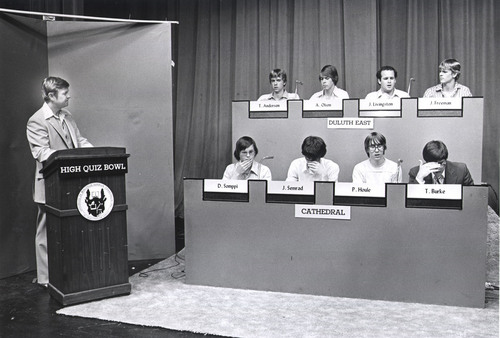
\includegraphics{qb/quizbowl}

	\end{columns}

\end{frame}

\begin{comment}

\begin{frame}[t]
	\frametitle{Sample Question 1}

With Leo Szilard, he invented a doubly-eponymous \only<2->{refrigerator with no moving parts. He did not take interaction with neighbors into account when formulating his theory of} \only<3->{heat capacity, so} \only<4->{Debye adjusted the theory for low temperatures. His} \only<4->{summation convention automatically sums repeated indices in tensor products. His name is attached to the A and B coefficients} \only<5->{for spontaneous and stimulated emission, the subject of one of his multiple groundbreaking 1905 papers. He further developed the model of statistics sent to him by} \only<6->{Bose to describe particles with integer spin. For 10 points, who is this German physicist best known for formulating the} \only<7->{special and general theories of relativity?} \\
\vspace{1cm}
\only<8->{ {\bf Albert \underline{Einstein}}}
\end{frame}

\end{comment}


\begin{frame}[t]
\frametitle{Sample Question}

One is Monte Carlo if at least half of the possible results for all x in a
\only<2->{language it says ``yes'' and ``no'' otherwise. One is called} \only<3->{unambiguous if for any $x$�there is at most one accepting computation. One is
called} \only<4->{oblivious if the position of the} \only<5->{cursor at the $t^{th}$
step depends only on the $t$ and the length of the input. One is} \only<6->{non-deterministic if its sets of next} \only<7->{states may contain more than one
element. For ten points, identify this model of} \only<8->{computation named for
an} \only<9->{English computer scientist.} \\
\only<10->{{\bf ANSWER: \underline{Turing} Machine (prompt on TM)}}


\end{frame}


\begin{frame}[t]
	\frametitle{Sample Question}
A letter from Vergnaud to Chomsky first made the argument that all \only<2->{DPs must have it.  Chomsky called IPs} \only<3->{faulty because its assignment in sentences with verbs like} \only<4->{``believe'' can change the specifier in a process called its} \only<5->{``exceptional marking''.  In Russian, the ending for the} \only<6->{instrumental one is} \only<7->{``om,'' and in German,} \only<8->{``des'' is an article for the genitive one.  For 10 points, name this} \only<9->{linguistic feature that signifies whether a noun is a} \only<10->{subject when it's nominative or an object when it's accusative.} \\
\vspace{.5cm}
\only<11->{ {\bf abstract \underline{case}}}

\only<12->{
  \begin{block}{Things to note}
    \begin{itemize}
    \item Pyramidality
      \iflong
    \item ``For ten points'' (FTP)
      \fi
      \end{itemize}
  \end{block}
}

\end{frame}

\begin{frame}
	\frametitle{Humans doing Incremental Classification}

	\begin{columns}
		\column{.5\linewidth}

		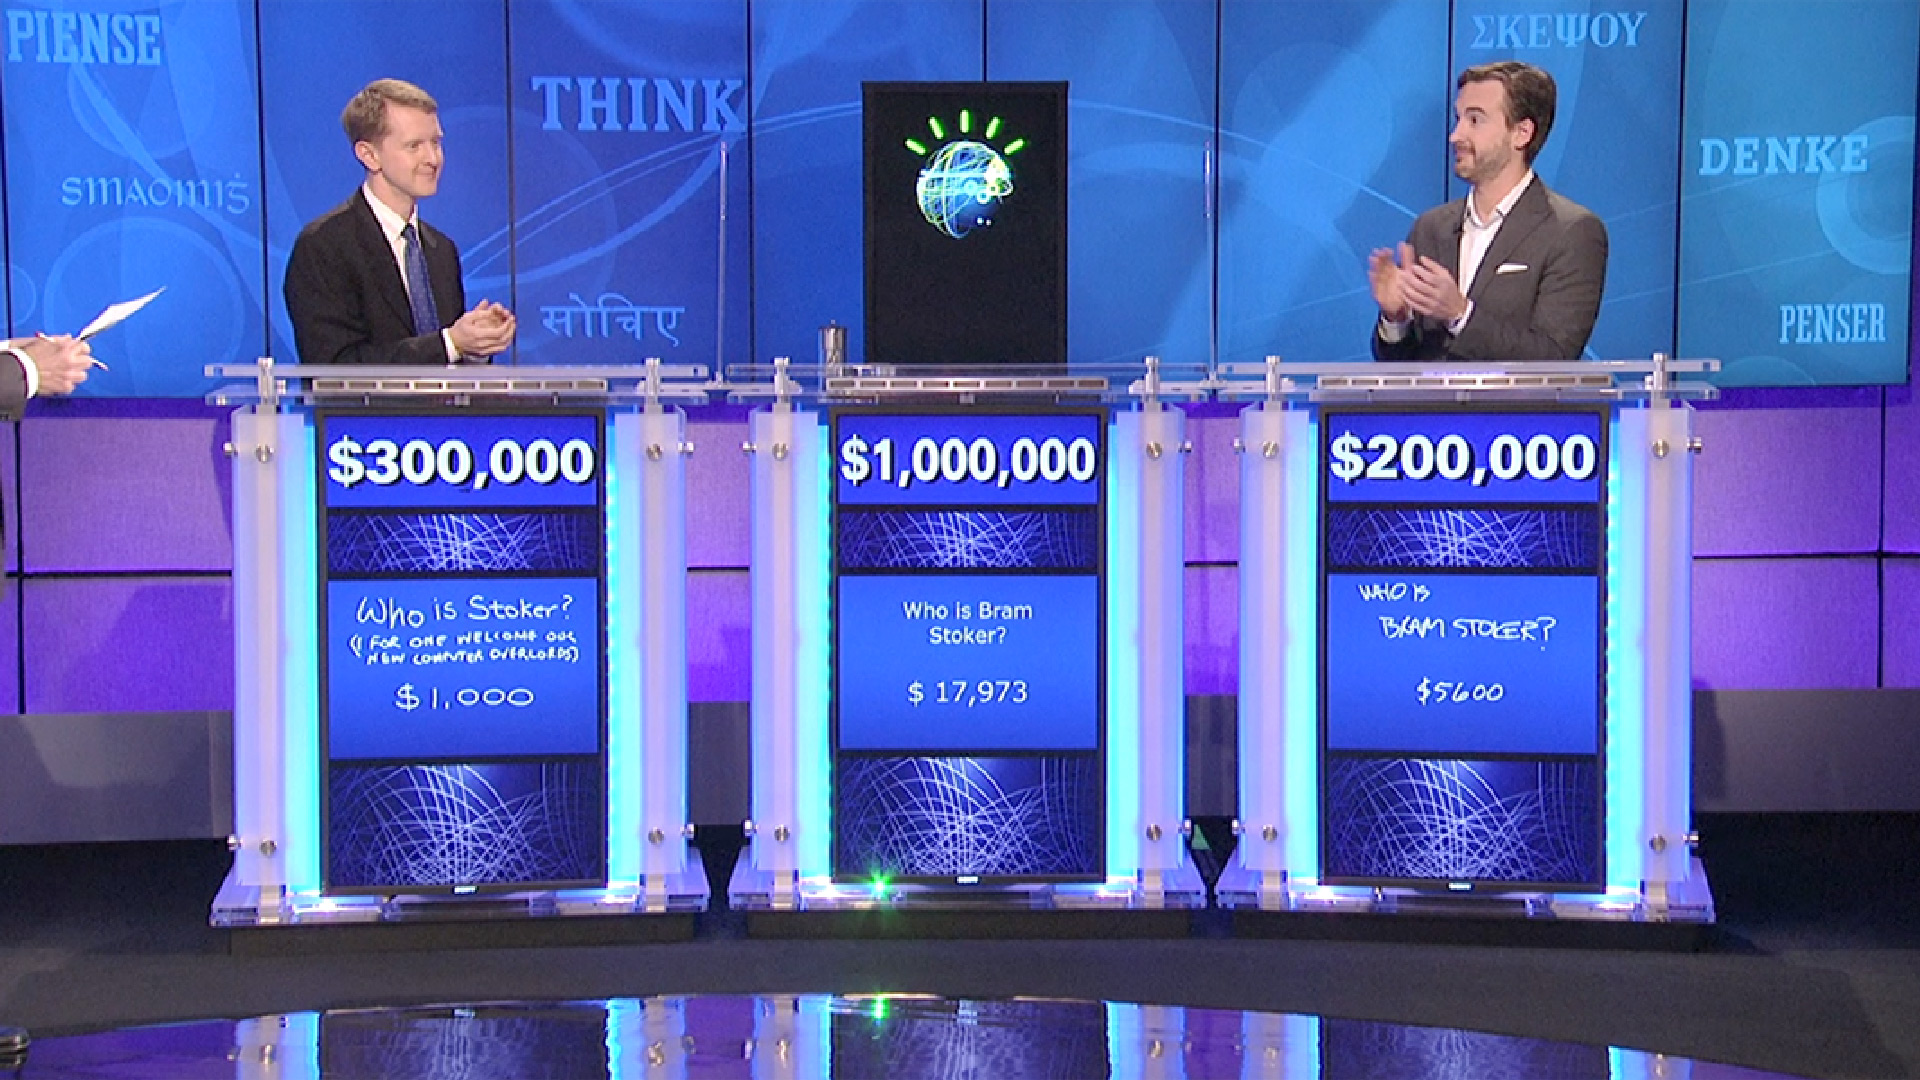
\includegraphics[width=1.0\linewidth]{qb/jeopardy}


		\column{.5\linewidth}
		\begin{itemize}
			\item This is {\bf not} Jeopardy \cite{ferruci-10}
			\item There are buzzers, but players can only buzz at the end of a question
			\item Doesn't discriminate knowledge
			\item Quiz bowl questions are pyramidal
		\end{itemize}

	\end{columns}

\end{frame}



\begin{frame}
	\frametitle{Humans doing Incremental Classification}

	\begin{itemize}
		\item Thousands of questions are written every year
		\item Large question databases
		\item Teams practice on these questions (some online, e.g. IRC)
		\item How can we use this process?
	\end{itemize}

\end{frame}


\section{Data Collection}

\begin{frame}

\frametitle{Interface}

\begin{columns}

	\column{0.5\linewidth}

	\begin{center}
		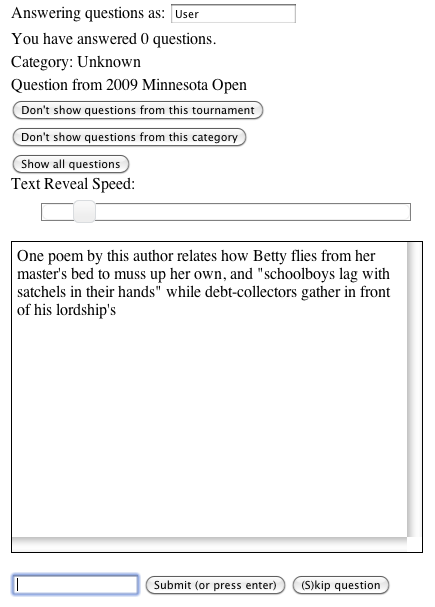
\includegraphics[width=0.9\linewidth]{qb/screenshot}
	\end{center}

	\column{0.5\linewidth}
	\only<1>{
	\begin{itemize}
		\item Users could ``veto'' categories or tournaments
		\item Questions presented in canonical order
		\item Approximate string matching (w/ override)
	\end{itemize}
	}

	\only<2>{
	\begin{itemize}
		\item Started on Amazon Mechanical Turk
		\item 7000 questions were answered in the first day
		\item Over 43000 questions were answered in the space of two weeks
		\item Total of 461 unique users
		\item Leaderboard to encourage users
	\end{itemize}
	}

\end{columns}
\end{frame}

\iflong

\begin{frame}
	\frametitle{Accuracy vs. Speed}

	\begin{center}
	  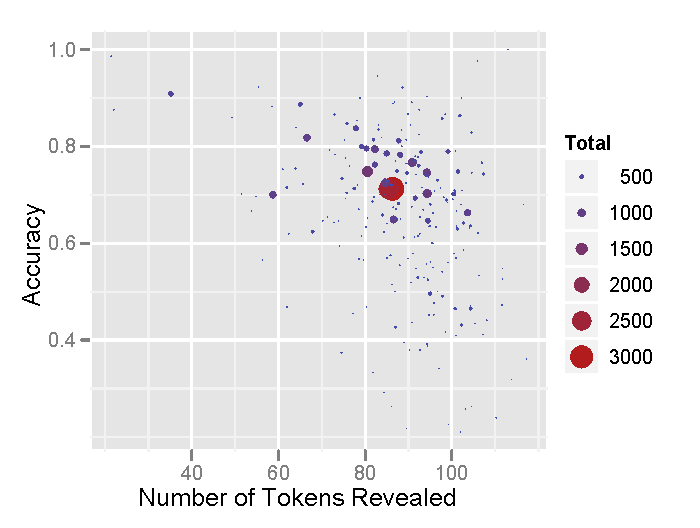
\includegraphics[width=0.9\linewidth]{qb/accuracy_vs_speed}
	  \end{center}

\end{frame}

\fi

\begin{frame}
	\begin{center}

\vspace{-.6cm}
\begin{figure}[tb]
\centering
\iflong
\subfigure[Buzzes over all Questions]{
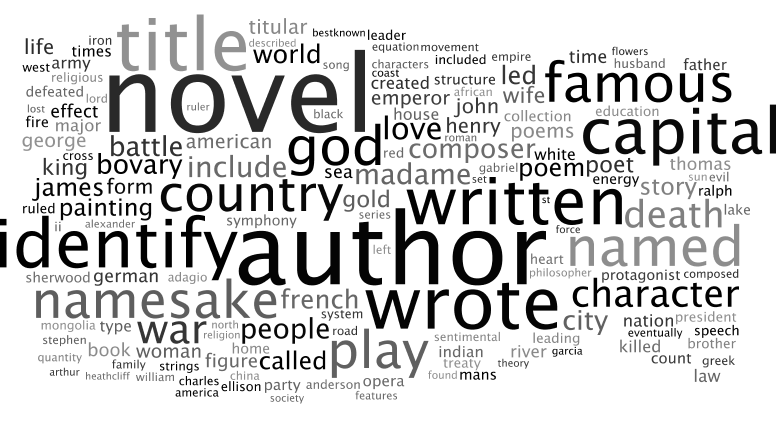
\includegraphics[width=0.6\linewidth]{qb/buzz_cloud}
\label{fig:buzz_cloud}
}
\fi
\subfigure[Wuthering Heights Question Text]{
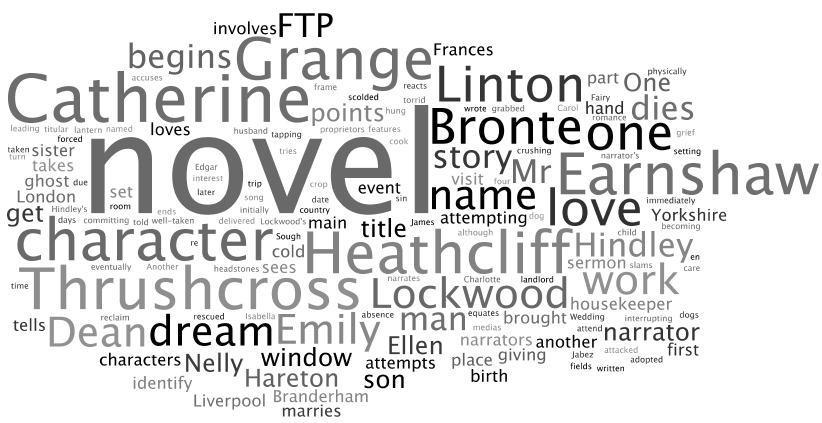
\includegraphics[width=0.45\linewidth]{qb/wuthering_heights_question}
\label{fig:wh_question}
}
\subfigure[Buzzes on Wuthering Heights]{
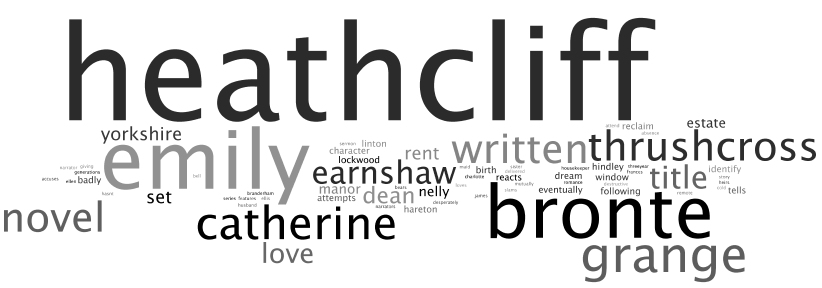
\includegraphics[width=0.45\linewidth]{qb/wuthering_heights_buzz}
\label{fig:wh_buzz}
}
\end{figure}


	\end{center}

\end{frame}

\iflong
	

\begin{frame}
	\frametitle{Learning which Features are Useful}

	\begin{itemize}
		\item Use how humans these data as a prior for supervised maxent model~\cite{daume-04}
		\item Prior for label $a$ and feature $f$ is a function of the number of buzzes $b$ and tf-idf~\cite{salton-68}
\begin{equation}
  \left[ \vphantom{\frac{a}{b}}\alpha \alert<4>{\ind{ b(a,f) > 0}} + \beta \alert<3>{ b(a,f)} + \gamma
  \right] \alert<2>{\mbox{tf-idf}(a,f)} .
\label{eq:meanweight}
\end{equation}
		\begin{itemize}
			\item $\alpha$, $\beta$, and $\gamma = 0$: na\"ive zero prior
			\item $\alpha$ and $\beta = 0$: linear transformation of the mean
			\item $\alpha$ and $\gamma = 0$: number of buzzes times tf-idf value of the features
		\end{itemize}

	\end{itemize}

\end{frame}

\begin{frame}
	\frametitle{Using buzzes as a prior}

\begin{equation*}
  \left[ \vphantom{\frac{a}{b}}\alpha \ind{ b(a,f) > 0} + \beta b(a,f) + \gamma
  \right] \mbox{tf-idf}(a,f) .
\end{equation*}

\begin{center}
\begin{tabular}{cccccc}
Answers & Weighting & $\alpha$ & $\beta$ & $\gamma$ & Error\footnote{Buzz and tf-idf computed on training data; grid search on dev data; error on test data} \\
\hline
\multirow{5}{*}{100} & zero & - & - & - & 0.22 \\
& tf-idf & - & - & 8.3 & 0.08 \\
&  buzz-binary & 10.7 & - & - & {\bf 0.06} \\
&  buzz-linear & - &  1.1 & - & 0.10 \\
& buzz-tier & - & 1.6 & 0.5 & 0.07 \\
\hline
\end{tabular}
\end{center}
\end{frame}



\fi
\section{Quiz Bowl Playing Robot}

\begin{frame}
	\frametitle{System for Incremental Classifiers}

	\begin{itemize}
		\item Treat this as a MDP
		\item Action: {\bf buzz} now or {\bf wait}
                     \pause
                    \begin{enumerate}
                  \item {\bf Content Model} is constantly generating guesses
                     \item {\bf Oracle} provides examples where it is correct
                   \item The {\bf Policy} generalizes to test data
                       \item {\bf Features} represent our state
                    \end{enumerate}
	\end{itemize}
\begin{block}{}
  \begin{center}
    \vspace{-.5cm}
    \begin{tabular}{cccc}
      \alert<3->{content model} & oracle & policy & features \\
    \end{tabular}
    \vspace{-.5cm}
  \end{center}
\end{block}
\end{frame}


\begin{frame}{Content Model}

\begin{block}{}
  \begin{center}
    \vspace{-.5cm}
    \begin{tabular}{cccc}
      \alert{content model} & oracle & policy & features \\
    \end{tabular}
    \vspace{-.5cm}
  \end{center}
\end{block}


  \begin{itemize}
   \item Bayesian generative model with answers as latent state
         \item Unambiguous Wikipedia pages
           \item Na\"ive Bayes
    \item Maintains posterior distribution over guesses
    \item Always has a guess of what it should answer
      \begin{itemize}
        \item policy will tell us when to trust it
       \end{itemize}

  \end{itemize}
\end{frame}

\begin{frame}{Oracle}
\begin{block}{}
  \begin{center}
    \vspace{-.5cm}
    \begin{tabular}{cccc}
      content model & \alert{oracle} & policy & features \\
    \end{tabular}
    \vspace{-.5cm}
  \end{center}
\end{block}
\begin{center}
  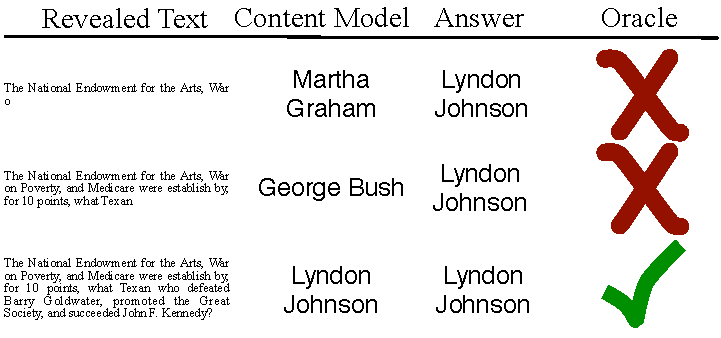
\includegraphics[width=0.8\linewidth]{qb/oracle}
\end{center}

\begin{itemize}
  \item As each token is revealed, look at content model's guess
    \item If it's right, positive instance; otherwise negative
      \item Nearly optimal policy to buzz whenever correct (upper bound)
\end{itemize}

\end{frame}

\begin{frame}{Policy}

\begin{block}{}
  \begin{center}
    \vspace{-.5cm}
    \begin{tabular}{cccc}
      content model & oracle & \alert{policy} & features \\
    \end{tabular}
    \vspace{-.5cm}
  \end{center}
\end{block}

 \begin{itemize}
    \item Mapping: state $\mapsto$ action
    \item Use oracle as example actions
    \item Learned as classifier \cite{langford-05}
    \item At test time, use the same features as for training
      \begin{itemize}
        \item Question text (so far)
        \item Guess
        \item Posterior distribution
        \item Change in posterior
      \end{itemize}
\end{itemize}

\end{frame}



\begin{frame}[t]{Features (by example)}

\only<1-3>{
\begin{block}{}
  \begin{center}
    \vspace{-.5cm}
    \begin{tabular}{cccc}
      content model & oracle & policy & \alert{features} \\
    \end{tabular}
    \vspace{-.5cm}
  \end{center}
\end{block}
\vspace{.5cm}
}

  \begin{columns}[T]
    \column{.3\linewidth}

    \only<1->{ 
\includegraphics[width=2\linewidth]{qb/feature_ex_l_1} \\ }
    \vspace{.5cm}
    \only<4->{ 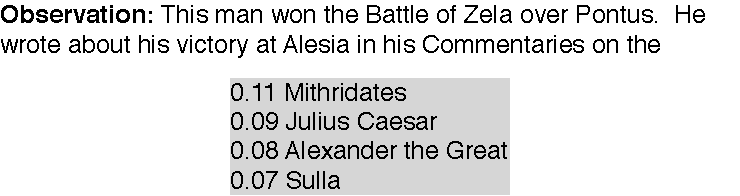
\includegraphics[width=2\linewidth]{qb/feature_ex_l_2}  \\ }
    \vspace{.5cm}
    \only<7->{ 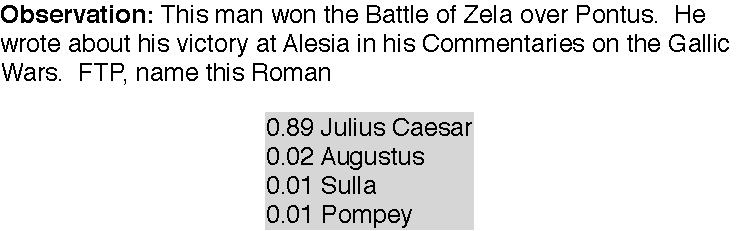
\includegraphics[width=2\linewidth]{qb/feature_ex_l_3}  \\ }


    \column{.68\linewidth}
    \vspace{-.5cm}
    \only<2->{ 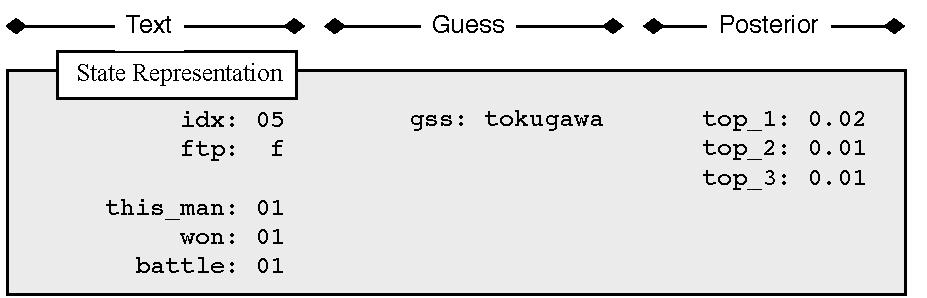
\includegraphics[width=.85\linewidth]{qb/feature_ex_r_1} \\ }
    \only<3->{ \vspace{-.5cm} \hspace{.5cm} 
\includegraphics[width=.1\linewidth]{qb/feature_ex_wait}  \\ }
    \only<5->{ 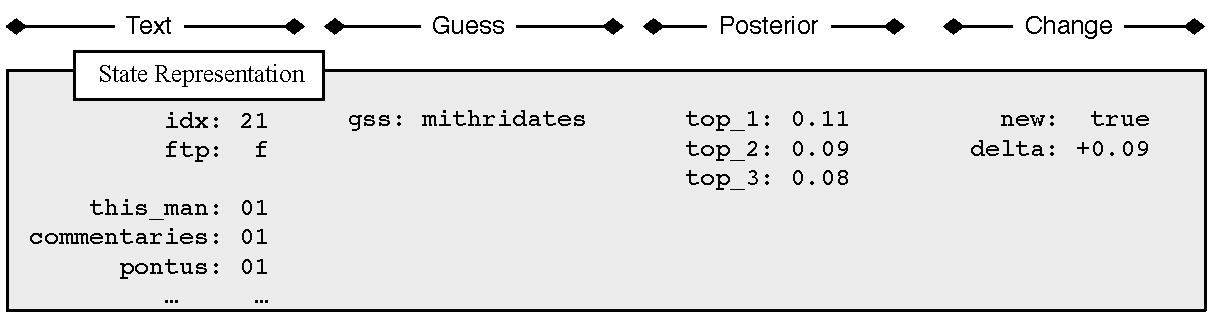
\includegraphics[width=\linewidth]{qb/feature_ex_r_2} \\ }
    \only<6->{ \vspace{-.5cm} \hspace{.5cm}
\includegraphics[width=.1\linewidth]{qb/feature_ex_wait}  \\ }
    \only<8->{ 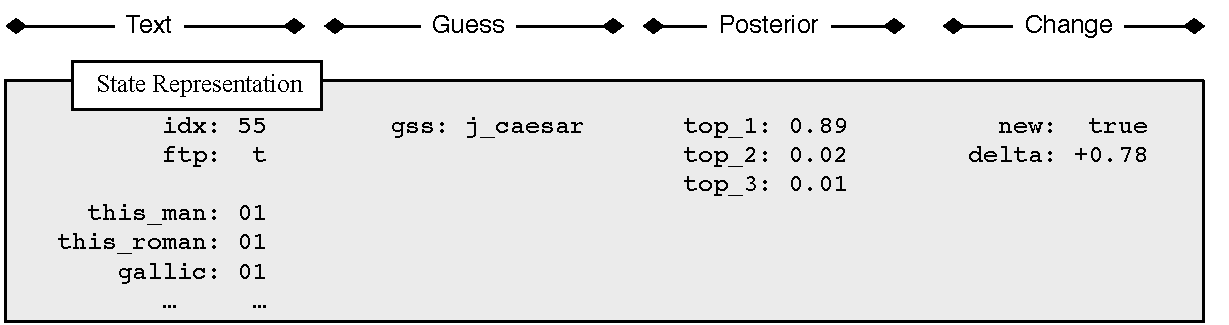
\includegraphics[width=\linewidth]{qb/feature_ex_r_3} \\ }
    \only<9->{ \vspace{-.5cm} \hspace{.5cm} 
\includegraphics[width=.1\linewidth]{qb/feature_ex_buzz}  \\ }
    \only<9->{Answer: {\bf Julius Caesar}}
  \end{columns}

\end{frame}



\begin{frame}{Simulating a Game}
		\begin{itemize}
			\item Present tokens incrementally to algorithm, see where it buzzes
			\item Compare to where humans buzzed in
			\item Payoff matrix (wrt Computer)
			\begin{center}
\begin{tabular}{lccr}
& Computer & Human & Payoff \\
\hline
1 & first and wrong & right & $-15$ \\
2 & --- & first and correct & $-10$ \\
3  & first and wrong & wrong & $-5$ \\
4 & first and correct & --- & $+10$ \\
5 & wrong & first and wrong & $+5$ \\
6 & right & first and wrong & $+15$ \\
\hline
\end{tabular}
			\end{center}
		\end{itemize}
\end{frame}

\iflong

\begin{frame}[t]
	\frametitle{Race Against the Machine}
	\begin{center}

\begin{tabular}{|ll|ccc|c|}
\hline
      &   & \multicolumn{3}{c|}{Human Scoring} & \\
Strategy&	Features & \alert<1>{Average} &	\alert<2>{Best}&	\alert<3>{Median} &	Token\\
\hline
\multirow{4}{*}{Classify}
& text & -8.72 & -10.04 & -6.50 & 40.36 \\
& +guess & -5.71 & -8.40 & -3.95 & 66.02 \\
& +pos & -4.13 & -7.56 & -2.70 & 67.97 \\
& \alert<5>{+change} & {\bf -4.02} & {\bf -7.41} & {\bf -2.63} & 77.33 \\
\hline
\alert<6>{Oracle} &  & 3.36 & 0.61 & 4.35 & 49.90 \\
\hline
                      & \alert<7>{all}             & -6.61         & -9.03         & -4.42 & 100.19 \\
                     & \alert<8>{ftp}              & -5.22         & -8.62         & -4.23 & 88.65 \\
Rapacious             &  \alert<9>{index$_{30}$}   & -7.89         & -8.71         & -6.41 & 32.23 \\
Baseline         &  \alert<9>{index$_{60}$ }       & -5.16         & {\bf -7.56}   & -3.71 & 61.90 \\
                      & \alert<9>{ index$_{90}$ }  & {\bf -5.02}   & -8.62         & {\bf -3.50} & 87.13 \\
\hline
\end{tabular}
	\end{center}
\vspace{-1cm}
% \only<4>{ \paragraph{token} Where the algorithm buzzed in.}
\only<6>{ \paragraph{Oracle} Best possible incremental strategy \emph{post hoc}}
\only<5>{ \paragraph{Classify} Incremental algorithms doing best, but not that well}
\only<7>{ \paragraph{all} This strategy waits until the end of the question and answers the best
  answer possible.}
\only<8>{ \paragraph{ftp} Waiting until when ``for 10 points'' is said, then giving the
    best answer possible.}
\only<9>{ \paragraph{index-n} Waiting until the first feature after the $n^{th}$ token has been processed, then giving the best answer possible.  }
\only<1> { \paragraph{average} For each human who answered a question, compare the positions and compute a reward.  Average them.}
\only<2> { \paragraph{best} For each question, take the human buzz position to be the the
  earliest that \emph{any} human buzzed in the question}
\only<3> { \paragraph{median} For each question, take the human buzz position to be the
  earliest position after 50\% of human buzzes appeared.}
\end{frame}


\else

\begin{frame}{Simulating a Game}

  \begin{itemize}
    \item What human actions to compare against?
      \invisible<1>{
      \begin{itemize}
        \item On each question, take the {\bf median} buzz (more in paper)
      \end{itemize}
      }
     \item Does it to better than obvious rapacious baselines?
      \invisible<-2>{
        \begin{itemize}
          \item Yes---experiments in paper
          \end{itemize}
        }
    \item How do features affect performance?
      \invisible<-3>{
      \begin{itemize}
        \item Nothing hurts, but only a handful help (details in paper)
      \end{itemize}
      }
  \end{itemize}

  \invisible<-4>{.}

\end{frame}


\begin{frame}{How does a na\"ive content model do?}
\begin{center}
\begin{tabular}{ll|c|c}
Strategy &  Model    &	Points &	Index\\
\hline
\multirow{4}{*}{Classify}
& na\"ive & -1.63 & 77.33 \\
& & & \\
& & & \\
& & & \\
\hline
\end{tabular}
\end{center}

\end{frame}

\fi



\iflong
\section{Hierarchical Bayesian Content Models}
\fi

\begin{frame}{What should the content model look like?}
	\begin{itemize}
		\item Should know what kinds of questions there are
                  \begin{itemize}
                    \item Humans do the same thing
                      \item Prevents crazy wrong answers (e.g. ``entropy'' for
                        ``Brahms'' when ``Schumann'' would be better)
                    \end{itemize}
		\item Should know how questions are structured
		\begin{itemize}
			\item Titles
			\item Quotes
                          \item Relationships
		\end{itemize}
                \pause
                 \item Add bigrams and categories to Bayesian model~\cite{wood-09}
	\end{itemize}

\iflong
\else
\pause

\vspace{-4cm}

  \begin{block}{Short story:}
    \begin{itemize}
      \item Models know universe of possible categories ({\bf cat}),
    \item How questions were structured ({\bf
      bigram})
    \item Will hopefully do better than ({\bf na\"ive}) model
      \end{itemize}
    \end{block}
\fi

\end{frame}

\iflong

\begin{frame}{Richer Content Models}

\begin{enumerate*}
  \item For each category $c$ of questions, draw a distribution over words
    \alert<4>{$\theta_c \sim \dir{\lambda_1 \theta_0}$}.
    \begin{itemize*}
   \alert<3>{ \item For each label $l$ in category $c$, draw a distribution over words
      $\theta_{l,c} \sim \dir{\lambda_2 \theta_c}$ }
   \alert<2>{   \item For each type $v$, draw a bigram distribution $\theta_{l,c,v} \sim
        \dir{\lambda_3 \theta_{l,c}}$ }
  \end{itemize*}
  \item Draw a distribution over labels $\phi \sim \dir{\alpha}$.
  \item For each question with category $c$ and $N$ words, draw answer $l \sim \mult{\phi}$:
    \begin{itemize*}
\footnotesize
      \item Assume $w_0 \equiv \mbox{\textsc{Start}}$
     \alert<1>{ \item Draw $w_n \sim \mult{\theta_{l,c,w_{n-1}}}$ for $n \in \{1 \dots N\}$ }
    \end{itemize*}
\end{enumerate*}

\only<5>{
 
\vspace{-4cm}

  \begin{block}{Short story:}
    \begin{itemize}
      \item Models know universe of possible categories ({\bf cat}),
    \item How questions were structured ({\bf
      bigram})
    \item Will hopefully do better than ({\bf na\"ive}) model
      \end{itemize}
    \end{block}
}

\end{frame}

\fi

\begin{frame}{Performance with rich content models}

\begin{center}
\iflong
\begin{tabular}{ll|ccc|c}
Strategy &  Model     &	Mean&	Best&	Median&	Index\\
\hline
\multirow{4}{*}{Classify}
& na\"ive & -4.02 & -7.41 & -2.63 & 77.33 \\
& cat & -1.69 & -5.22 & 0.12 & 67.97 \\
& bigram & -3.80 & -7.66 & -2.51 & 78.69 \\
& bgrm+cat & {\bf -0.86} & {\bf -4.46} & {\bf 0.83} & 63.42 \\
\hline
\multirow{4}{*}{Oracle}
& naive & 3.36 & 0.61 & 4.35 & 49.90 \\
& cat & 4.48 & 1.64 & 5.47 & 47.88 \\
& bigram & 3.58 & 0.87 & 4.61 & 49.34 \\
& bgrm+cat & {\bf 4.67} & {\bf 1.99} & {\bf 5.74} & 46.49 \\
\hline
\end{tabular}

\else

\begin{tabular}{ll|c|c}
Strategy &  Model    &	Points &	Index\\
\hline
\multirow{4}{*}{Classify}
& na\"ive & -1.63 & 77.33 \\
& \invisible<-1>{ cat} & \invisible<-1>{ 0.12} & \invisible<-1>{ 67.97} \\
& \invisible<-2>{ bigram} & \invisible<-2>{-1.51} & \invisible<-2>{ 78.69} \\
& \invisible<-3>{ bgrm+cat} & \invisible<-3>{{\bf 0.83}} & \invisible<-3>{ 63.42} \\
\hline
\end{tabular}

\fi
\end{center}


\only<5>{

\vspace{-3cm}

\begin{block}{Beating median player}
  \begin{itemize}
    \item As far as we got (so far)
      \item But we're still not beating best players
        \item Where can we improve?
    \end{itemize}
\end{block}

}

\end{frame}

\iflong

\begin{frame}[t]

\frametitle{Error Analysis}

\begin{columns}

	\column{.4 \linewidth}
        \only<5-> {

		\begin{itemize}
			\item \alert<5> { Too slow }
			\item \alert<6> {Coreference \cite{haghighi-07} and correct question
type \cite{moldovan-00}}
			\item \alert<7> {Not enough information / not weighting later clues higher }
		\end{itemize}

}

	\column{.6 \linewidth}

		\begin{center}
			\only<1>{  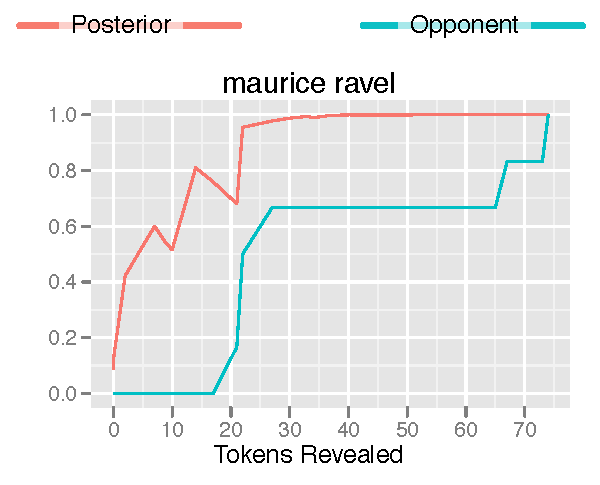
\includegraphics[width=.9\linewidth]{qb/real_question_ravel_0} \\ }
			\only<2>{  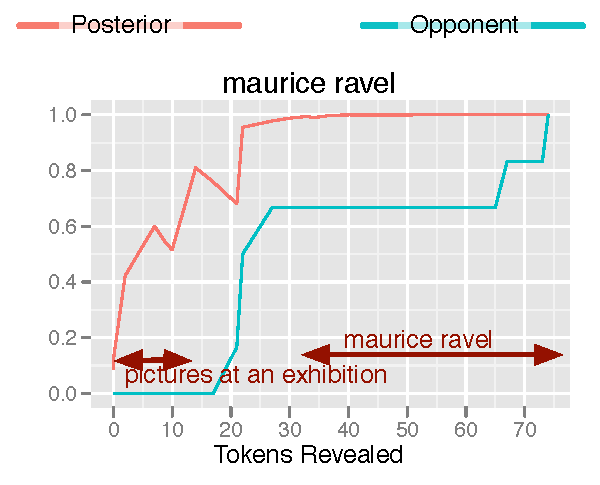
\includegraphics[width=.9\linewidth]{qb/real_question_ravel_1} \\ }
			\only<3>{  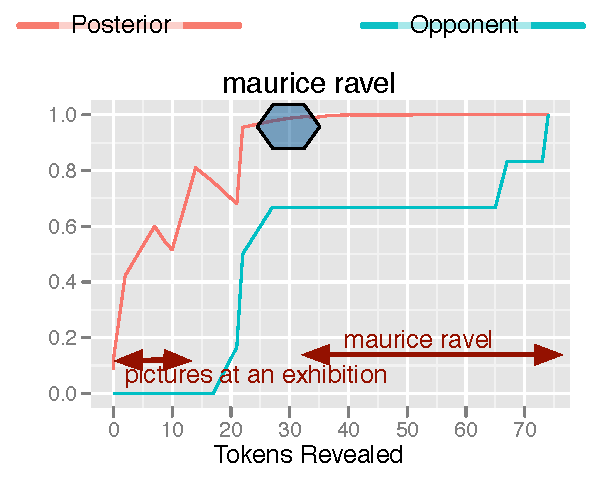
\includegraphics[width=.9\linewidth]{qb/real_question_ravel_2}
                          \\ }
			\only<4-5>{  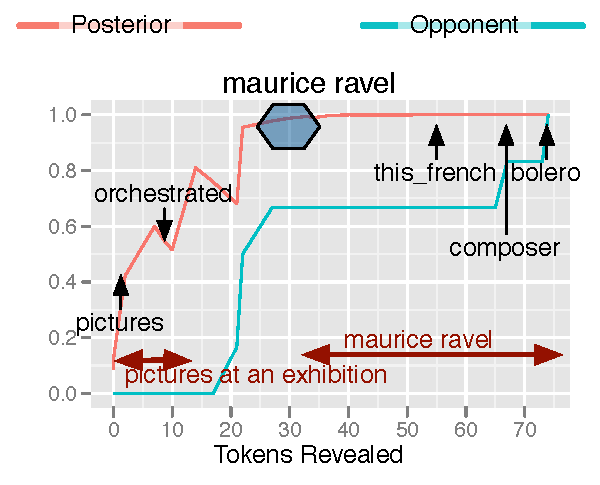
\includegraphics[width=.9\linewidth]{qb/real_question_ravel_3} \\ }
			\only<6>{  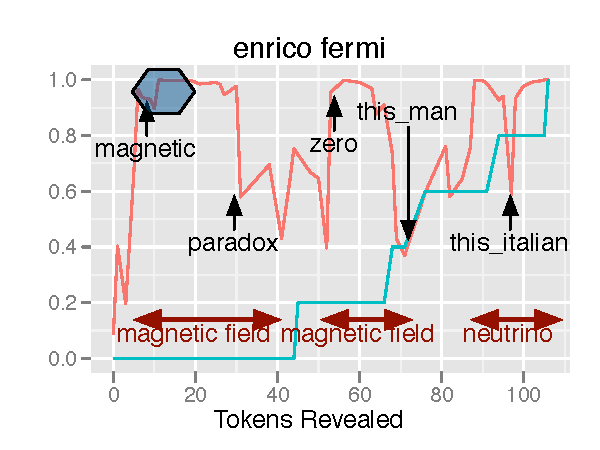
\includegraphics[width=.9\linewidth]{qb/real_question_fermi} \\ }
			\only<7>{  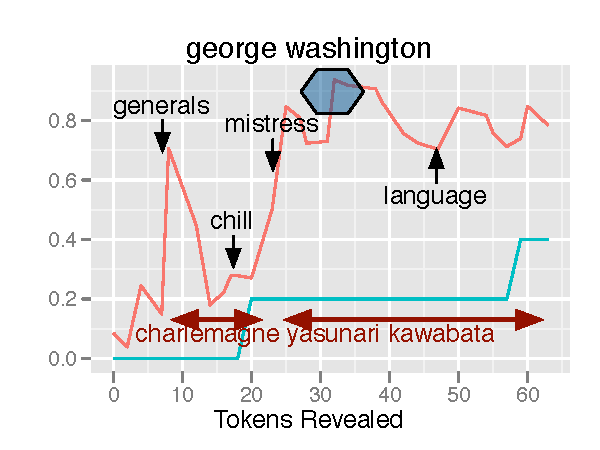
\includegraphics[width=.9\linewidth]{qb/real_question_washington} \\ }
			\only<2>{ 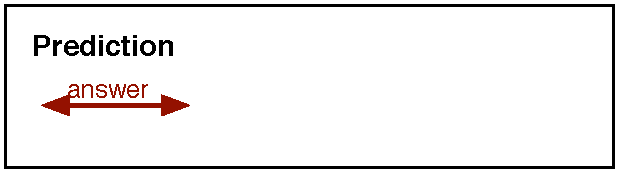
\includegraphics[width=.9\linewidth]{qb/real_question_key_0} }
			\only<3>{ 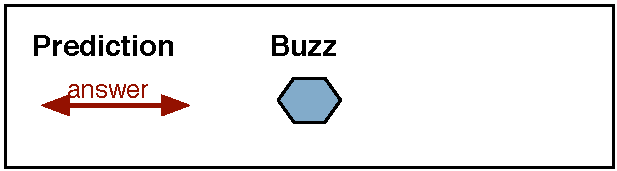
\includegraphics[width=.9\linewidth]{qb/real_question_key_1} }
			\only<4->{ 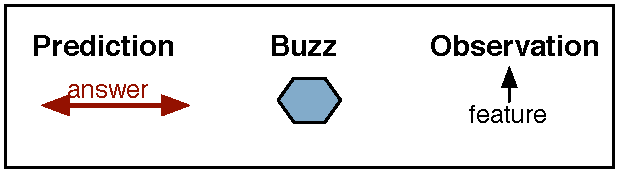
\includegraphics[width=.9\linewidth]{qb/real_question_key_2} }
		\end{center}
\end{columns}

\end{frame}

\else

\begin{frame}{Error Analysis}
  \begin{itemize}
    \item Simple stuff: Too slow
    \item Coreference \cite{haghighi-07} / question type \cite{moldovan-00}: Answering ``electric field'' for ``Enrico
      Fermi''
    \item Not enough data: Answering ``Yasunari Kawabata'' for ``George Washington''
  \end{itemize}
\end{frame}

\fi

\section{Why should you use QB data?}

\begin{frame}{Summarization / Paraphrase}

\begin{itemize}
  \item Clues in quiz bowl questions are structured in \emph{increasing} order of importance
  \item Questions with same label are each structured summaries
    \begin{itemize}
      \item First clues are diverse
      \item Last clues are ``cannonical''
      \end{itemize}
  \item Thousands of different labels, some with hundreds of relevant questions
\end{itemize}

\end{frame}

\begin{frame}{Summarization / Paraphrase}
{\bf Choson Dynasty}
\begin{columns}
  \column{.45\linewidth}
  \begin{block}{First Clues}
    \begin{itemize}
    \item One tomb of a king \only<1>{from this region is named for the depiction of a eight-legged, ``Heavenly'' horse found there.} \invisible<1>{\dots}
    \item During this dynasty \only<2>{, a monk of the Son sect helped secure the release of over 3,000 prisoners of war.} \invisible<2>{\dots}
    \item Prince Sado of \only<3>{this dynasty was executed by being shut in a rice box, and its cloth tax was decreased by the Kyunyok Law.} \invisible<3>{\dots}
    \item During this dynasty, a Catholic \only<4>{scholar developed a philosophy of the rights of the people that is classified as part of the ``practical learning'' modernization movement known as Silhak.} \invisible<4>{\dots}
      \end{itemize}
  \end{block}
  \column{.45\linewidth}
  \begin{block}{Last Clues}
    \begin{itemize}
    \item Name this successor of the Goryeo \only<5>{Dynasty which ruled Korea for over five hundred years.} \invisible<5>{\dots}
    \item Name this dynasty that ruled Korea \only<6>{until annexed by Japan in 1910.} \invisible<6>{\dots}
    \item Name this dynasty which succeeded the Koryo, \only<7>{the longest lasting dynasty of Korea.} \invisible<7>{\dots}
    \item \only<8>{The successor of the Koryo dynasty, for 10 points,}\only<-7>{\dots} was what final imperial dynasty of Korea?
     \end{itemize}
  \end{block}

\end{columns}

\end{frame}

\begin{frame}{Coreference / Hypernym Extraction}

\begin{itemize}
  \item Good style in quiz bowl question requires all references to refer to the answer
  \item Forces diverse range in allowable references
\end{itemize}

\pause

\begin{block}{Hanseatic League}
\alert<3>{This entity} made a military pact known as the Tohopesate, and \alert<3>{it} was harassed by forces of Klaus Stortebeker, the leader of the Likedeelers, which were successors of pirates known as the Victual Brothers. After the humiliating Peace of Vordingborg, \alert<3>{this group} forced Valdemar IV of Denmark to sign the Treaty of Stralsund. The Peterhof in Novgorod and Steelyard in London are notable examples of Kontores established by \alert<3>{this polity}, although \alert<3>{its} power faded as the Swedish Empire lessened the importance of cities such as Visby and Lubeck. For 10 points, name \alert<3>{this Northern European trading league} which controlled the Baltic Sea.
\end{block}

\end{frame}

\iflong
	
\section{Conclusion and Future Steps}



\begin{frame}
	\frametitle{Next: Richer content models}
	\begin{itemize}
		\item Look at anaphors explicitly with local context (e.g. ``plug in'')
		\item More data
		\item Link structure in Wikipedia (e.g., redirects)
		\item Lookahead
	\end{itemize}
\end{frame}

\begin{frame}
	\frametitle{Next: Richer interactions}
		\begin{itemize}
			\item Currently users competing against themselves
			\item But how you play depends on opponents
			\item Rollout of strategies?~\cite{tesauro-96}
			\item Better theoretical grounding~\cite{li-08}
			\item More complicated interface
			\item Game theory to estimate policies
			\item More fun
		\end{itemize}
\end{frame}

\begin{frame}
	\frametitle{Next: Linguistic effects}
		\begin{itemize}
			\item Posterior over answers and latent structure
			\item Can we capture interaction with syntax (e.g. tweaking sentence)
			\item Way of validating psycholinguistic theories about surprisal
		\end{itemize}
\end{frame}

\begin{frame}{Simultaneous Translation}
  \centering
  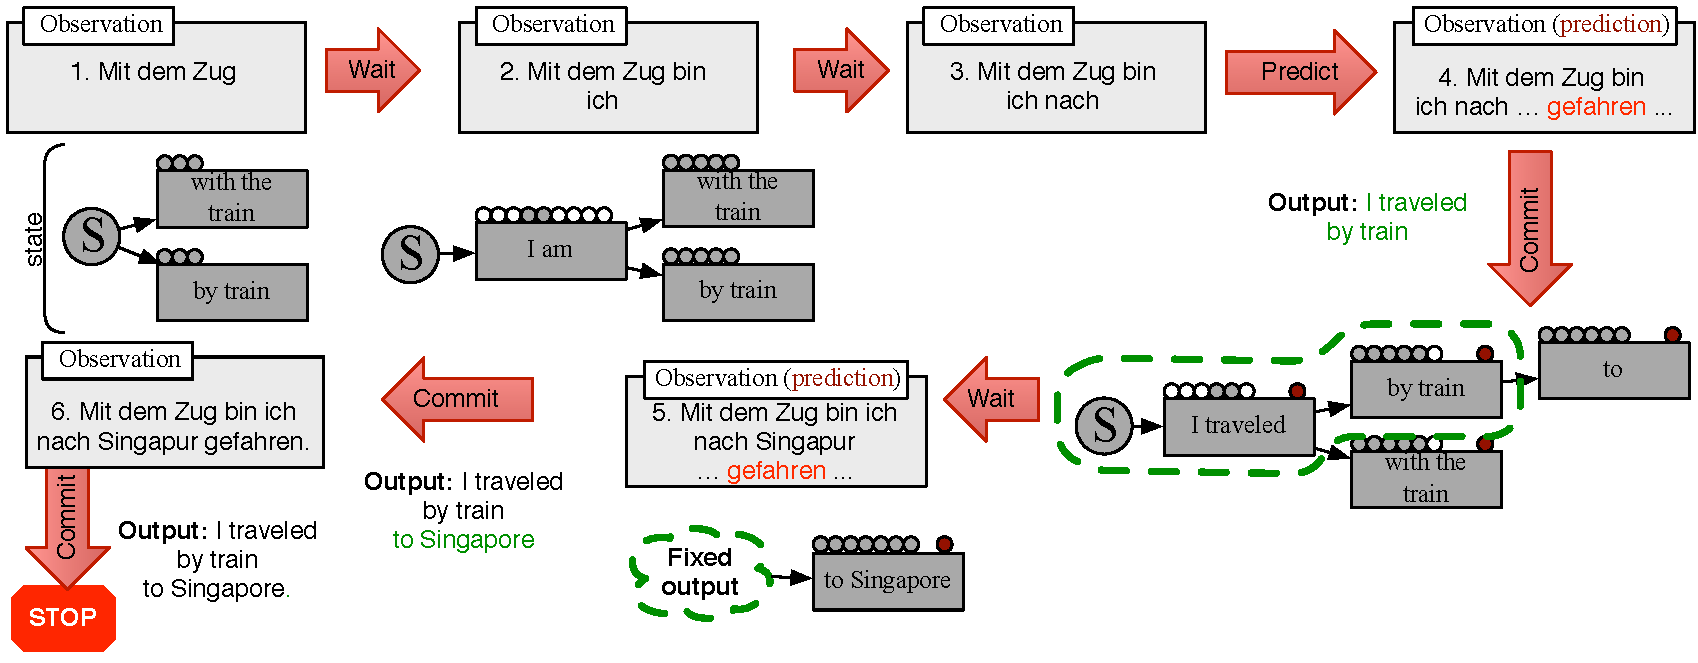
\includegraphics[width=1.0\linewidth]{qb/incremental_translation}
\end{frame}

\begin{frame}

	\frametitle{Recap}

	\begin{itemize}
			\item Fun and useful for users
			\item Improves batch learning
			\item Learning incremental classification by example
	\end{itemize}
\end{frame}

\else
	\begin{frame}{Conclusion and Future Steps}
	\begin{itemize}
		\item Quiz Bowl
		\begin{itemize}
			\item Fun
			\item Lots of data: \url{http://umiacs.umd.edu/~jbg/qb}
			\item Connected with many NLP and ML problems
                        \item Annotating coreference
		\end{itemize}
		\item Better Models
		\begin{itemize}
			\item Using RNNs to incorporate syntax
			\item Strategies for different opponents
                        \item Scaling up
		\end{itemize}
	\end{itemize}
	\end{frame}
\fi

\frame{

\huge Questions?

}


\iflong

\else



\begin{frame}
	\frametitle{Learning which Features are Useful}

	\begin{itemize}
		\item Use how humans these data as a prior for supervised maxent model~\cite{daume-04}
		\item Prior for label $a$ and feature $f$ is a function of the number of buzzes $b$ and tf-idf~\cite{salton-68}
\begin{equation}
  \left[ \vphantom{\frac{a}{b}}\alpha \alert<4>{\ind{ b(a,f) > 0}} + \beta \alert<3>{ b(a,f)} + \gamma
  \right] \alert<2>{\mbox{tf-idf}(a,f)} .
\label{eq:meanweight}
\end{equation}
		\begin{itemize}
			\item $\alpha$, $\beta$, and $\gamma = 0$: na\"ive zero prior
			\item $\alpha$ and $\beta = 0$: linear transformation of the mean
			\item $\alpha$ and $\gamma = 0$: number of buzzes times tf-idf value of the features
		\end{itemize}

	\end{itemize}

\end{frame}

\begin{frame}
	\frametitle{Using buzzes as a prior}

\begin{equation*}
  \left[ \vphantom{\frac{a}{b}}\alpha \ind{ b(a,f) > 0} + \beta b(a,f) + \gamma
  \right] \mbox{tf-idf}(a,f) .
\end{equation*}

\begin{center}
\begin{tabular}{cccccc}
Answers & Weighting & $\alpha$ & $\beta$ & $\gamma$ & Error\footnote{Buzz and tf-idf computed on training data; grid search on dev data; error on test data} \\
\hline
\multirow{5}{*}{100} & zero & - & - & - & 0.22 \\
& tf-idf & - & - & 8.3 & 0.08 \\
&  buzz-binary & 10.7 & - & - & {\bf 0.06} \\
&  buzz-linear & - &  1.1 & - & 0.10 \\
& buzz-tier & - & 1.6 & 0.5 & 0.07 \\
\hline
\end{tabular}
\end{center}
\end{frame}




\begin{frame}[t]
	\frametitle{Race Against the Machine}
	\begin{center}

\begin{tabular}{|ll|ccc|c|}
\hline
      &   & \multicolumn{3}{c|}{Human Scoring} & \\
Strategy&	Features & \alert<1>{Average} &	\alert<2>{Best}&	\alert<3>{Median} &	Token\\
\hline
\multirow{4}{*}{Classify}
& text & -8.72 & -10.04 & -6.50 & 40.36 \\
& +guess & -5.71 & -8.40 & -3.95 & 66.02 \\
& +pos & -4.13 & -7.56 & -2.70 & 67.97 \\
& \alert<5>{+change} & {\bf -4.02} & {\bf -7.41} & {\bf -2.63} & 77.33 \\
\hline
\alert<6>{Oracle} &  & 3.36 & 0.61 & 4.35 & 49.90 \\
\hline
                      & \alert<7>{all}             & -6.61         & -9.03         & -4.42 & 100.19 \\
                     & \alert<8>{ftp}              & -5.22         & -8.62         & -4.23 & 88.65 \\
Rapacious             &  \alert<9>{index$_{30}$}   & -7.89         & -8.71         & -6.41 & 32.23 \\
Baseline         &  \alert<9>{index$_{60}$ }       & -5.16         & {\bf -7.56}   & -3.71 & 61.90 \\
                      & \alert<9>{ index$_{90}$ }  & {\bf -5.02}   & -8.62         & {\bf -3.50} & 87.13 \\
\hline
\end{tabular}
	\end{center}
\vspace{-1cm}
% \only<4>{ \paragraph{token} Where the algorithm buzzed in.}
\only<6>{ \paragraph{Oracle} Best possible incremental strategy \emph{post hoc}}
\only<5>{ \paragraph{Classify} Incremental algorithms doing best, but not that well}
\only<7>{ \paragraph{all} This strategy waits until the end of the question and answers the best
  answer possible.}
\only<8>{ \paragraph{ftp} Waiting until when ``for 10 points'' is said, then giving the
    best answer possible.}
\only<9>{ \paragraph{index-n} Waiting until the first feature after the $n^{th}$ token has been processed, then giving the best answer possible.  }
\only<1> { \paragraph{average} For each human who answered a question, compare the positions and compute a reward.  Average them.}
\only<2> { \paragraph{best} For each question, take the human buzz position to be the the
  earliest that \emph{any} human buzzed in the question}
\only<3> { \paragraph{median} For each question, take the human buzz position to be the
  earliest position after 50\% of human buzzes appeared.}
\end{frame}


\begin{frame}{Richer Content Models}

\begin{enumerate*}
  \item For each category $c$ of questions, draw a distribution over words
    \alert<4>{$\theta_c \sim \dir{\lambda_1 \theta_0}$}.
    \begin{itemize*}
   \alert<3>{ \item For each label $l$ in category $c$, draw a distribution over words
      $\theta_{l,c} \sim \dir{\lambda_2 \theta_c}$ }
   \alert<2>{   \item For each type $v$, draw a bigram distribution $\theta_{l,c,v} \sim
        \dir{\lambda_3 \theta_{l,c}}$ }
  \end{itemize*}
  \item Draw a distribution over labels $\phi \sim \dir{\alpha}$.
  \item For each question with category $c$ and $N$ words, draw answer $l \sim \mult{\phi}$:
    \begin{itemize*}
\footnotesize
      \item Assume $w_0 \equiv \mbox{\textsc{Start}}$
     \alert<1>{ \item Draw $w_n \sim \mult{\theta_{l,c,w_{n-1}}}$ for $n \in \{1 \dots N\}$ }
    \end{itemize*}
\end{enumerate*}

\only<5>{
 
\vspace{-4cm}

  \begin{block}{Short story:}
    \begin{itemize}
      \item Models know universe of possible categories ({\bf cat}),
    \item How questions were structured ({\bf
      bigram})
    \item Will hopefully do better than ({\bf na\"ive}) model
      \end{itemize}
    \end{block}
}

\end{frame}

\begin{frame}[t]

\frametitle{Error Analysis}

\begin{columns}

	\column{.4 \linewidth}
        \only<5-> {

		\begin{itemize}
			\item \alert<5> { Too slow }
			\item \alert<6> {Coreference \cite{haghighi-07} and correct question
type \cite{moldovan-00}}
			\item \alert<7> {Not enough information / not weighting later clues higher }
		\end{itemize}

}

	\column{.6 \linewidth}

		\begin{center}
			\only<1>{  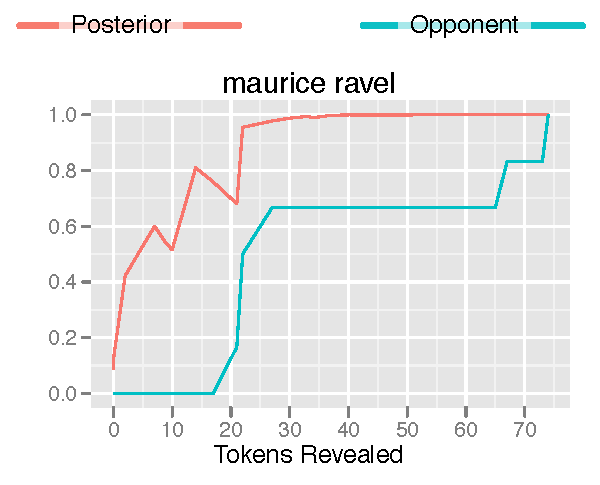
\includegraphics[width=.9\linewidth]{qb/real_question_ravel_0} \\ }
			\only<2>{  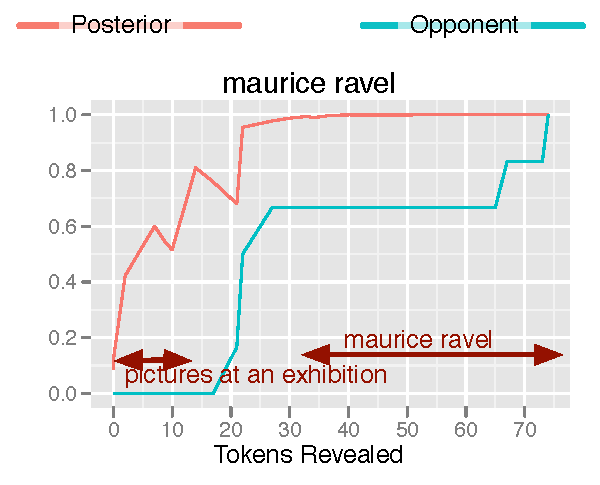
\includegraphics[width=.9\linewidth]{qb/real_question_ravel_1} \\ }
			\only<3>{  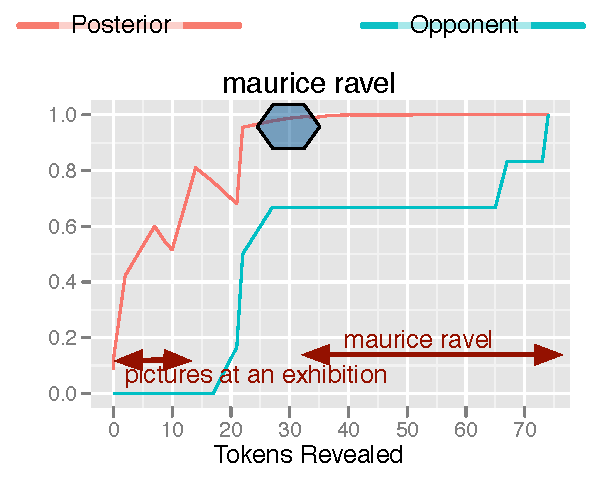
\includegraphics[width=.9\linewidth]{qb/real_question_ravel_2}
                          \\ }
			\only<4-5>{  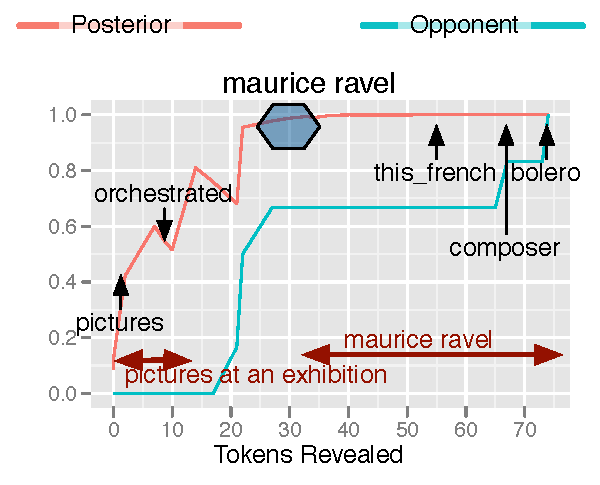
\includegraphics[width=.9\linewidth]{qb/real_question_ravel_3} \\ }
			\only<6>{  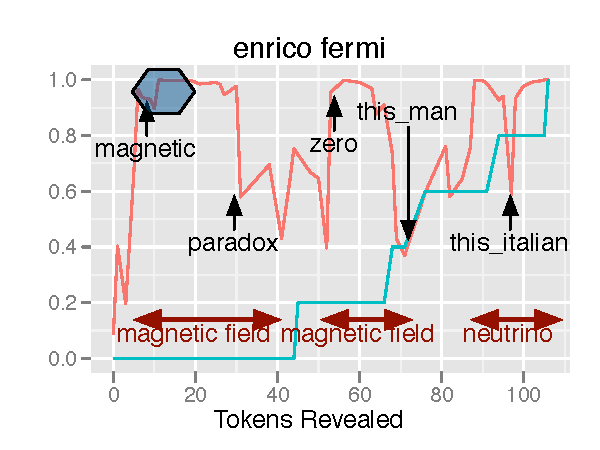
\includegraphics[width=.9\linewidth]{qb/real_question_fermi} \\ }
			\only<7>{  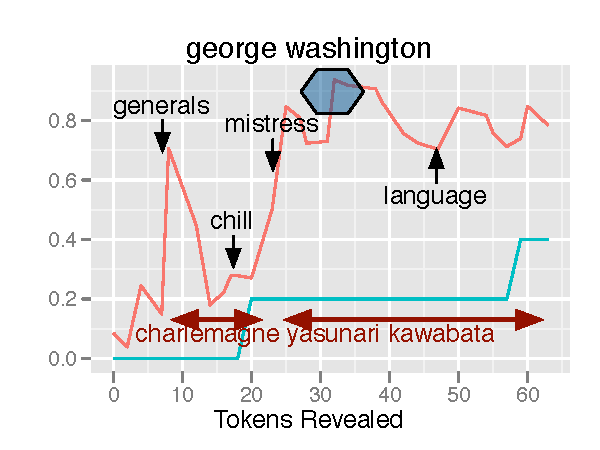
\includegraphics[width=.9\linewidth]{qb/real_question_washington} \\ }
			\only<2>{ 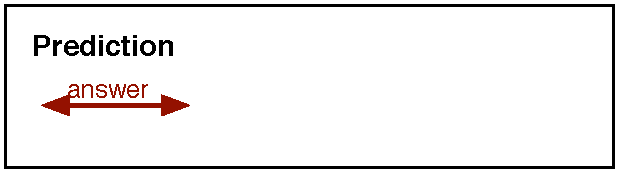
\includegraphics[width=.9\linewidth]{qb/real_question_key_0} }
			\only<3>{ 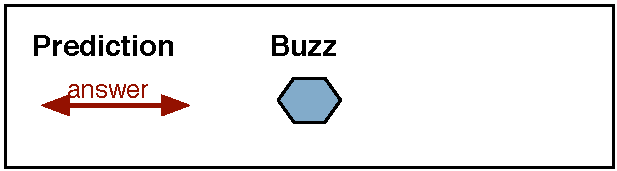
\includegraphics[width=.9\linewidth]{qb/real_question_key_1} }
			\only<4->{ 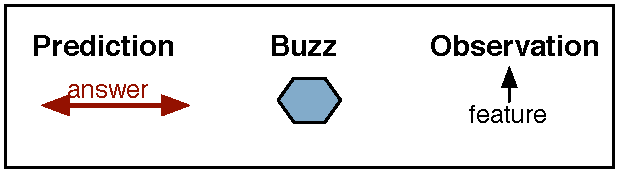
\includegraphics[width=.9\linewidth]{qb/real_question_key_2} }
		\end{center}
\end{columns}

\end{frame}


\fi


\begin{frame}

\frametitle{Logistic Regression}

\begin{tabular}{rrrrr}
  \hline
 & Estimate & Std. Error & z value & Pr($>$$|$z$|$) \\
  \hline
(Intercept) & -2.6200 & 0.0368 & -71.10 & 0.0000 \\
  Tokens revealed & 0.0229 & 0.0001 & 214.00 & 0.0000 \\
  ``ftp'' seen & 0.6677 & 0.0083 & 80.73 & 0.0000 \\
  Years after 2000 & -0.0005 & 0.0000 & -11.53 & 0.0000 \\
  Biology & -0.8975 & 0.0417 & -21.52 & 0.0000 \\
  Chemistry & -0.0323 & 0.0398 & -0.81 & 0.4171 \\
  Earth Science & -0.5980 & 0.1085 & -5.51 & 0.0000 \\
  Fine Arts & -0.6800 & 0.0372 & -18.29 & 0.0000 \\
  History & -0.5083 & 0.0374 & -13.61 & 0.0000 \\
  Literature & -0.6133 & 0.0368 & -16.65 & 0.0000 \\
  Mathematics & -0.5810 & 0.0530 & -10.95 & 0.0000 \\
  Other & -1.2591 & 0.0773 & -16.29 & 0.0000 \\
  Physics & -0.7292 & 0.0405 & -18.02 & 0.0000 \\
  Social Studies & -0.5607 & 0.0369 & -15.18 & 0.0000 \\
   \hline
\end{tabular}

\end{frame}

\begin{frame}
	\frametitle{Incremental Classification}
	\begin{block}{When to buzz?}
	\begin{equation}
  \mbox{Q}(X_n^{\mbox{new}}) =  \mbox{R}  \left(X_n^{\mbox{old}}\right) -
  \mbox{R}\left(X_n^{\mbox{old}} \cup
  X_n^{\mbox{new}}\right) - \mbox{\textsc{Waiting-Cost}}\left(X_n^{\mbox {new}}\right),
\label{eq:util}
\end{equation}
where the R is the expected reward given your best guess $\mbox{MC-Cost}(X_n) = $
\begin{equation*}
\alert<2>{\e{X_n}{ \max_{i} \rho p(z_n = i | X) + \sum_{j \not = i} \omega p(z_n = j | X)  }},
\end{equation*}
	\end{block}

\end{frame}

\begin{frame}
\bibliographystyle{acl}
\tiny
\bibliography{journal-full,jbg}
\end{frame}


\end{document}